\section[Process hacker]{Process hacker}

The Process Hacker \cite{processhacker} is an open-source project maintained by
Wen Jia Liu and Steven G. The goal of this project is to give the user a tool
to monitor system resources, debug software, and detect malware. Process Hacker
has a graphical user interface to inspect processes, network connections, file
access. Process Hacker also uses a kernel driver to capture stack traces,
enumerating process handler more efficiently, retrieving names for file
handlers and EtwRegistration objects, and setting handle attributes.

Process hacker does not use any forensics methods to detect malware, but either
using more verbose information into the system to let the user know what
processes are doing.


\begin{figure}[h]
  \centering
  \caption{Process Hacker}
  \label{fig:processhacker}
  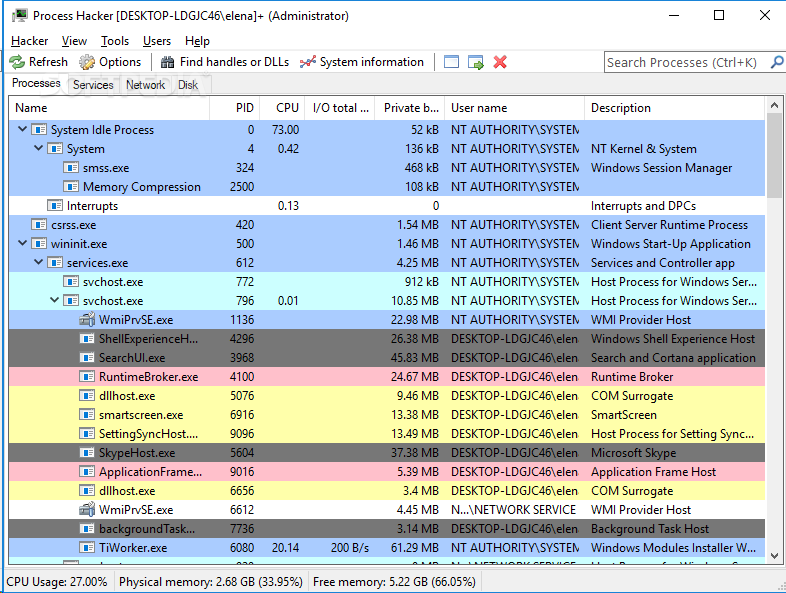
\includegraphics[scale=0.7]{images/processhacker.png}
\end{figure}
